\documentclass{tufte-handout}

%\geometry{showframe}% for debugging purposes -- displays the margins

\usepackage{amsmath}

% Set up the images/graphics package
\usepackage{graphicx}
\setkeys{Gin}{width=\linewidth,totalheight=\textheight,keepaspectratio}
\graphicspath{{graphics/}}

\title{Carbohydrate Structure}
\author{Olivia S. Anderson and Dave Bridges}
\date{}  % if the \date{} command is left out, the current date will be used

% The following package makes prettier tables.  We're all about the bling!
\usepackage{booktabs}

% The units package provides nice, non-stacked fractions and better spacing
% for units.
\usepackage{units}

% The fancyvrb package lets us customize the formatting of verbatim
% environments.  We use a slightly smaller font.
\usepackage{fancyvrb}
\fvset{fontsize=\normalsize}

% Small sections of multiple columns
\usepackage{multicol}

% Provides paragraphs of dummy text
\usepackage{lipsum}

% These commands are used to pretty-print LaTeX commands
\newcommand{\doccmd}[1]{\texttt{\textbackslash#1}}% command name -- adds backslash automatically
\newcommand{\docopt}[1]{\ensuremath{\langle}\textrm{\textit{#1}}\ensuremath{\rangle}}% optional command argument
\newcommand{\docarg}[1]{\textrm{\textit{#1}}}% (required) command argument
\newenvironment{docspec}{\begin{quote}\noindent}{\end{quote}}% command specification environment
\newcommand{\docenv}[1]{\textsf{#1}}% environment name
\newcommand{\docpkg}[1]{\texttt{#1}}% package name
\newcommand{\doccls}[1]{\texttt{#1}}% document class name
\newcommand{\docclsopt}[1]{\texttt{#1}}% document class option name


\begin{document}
\maketitle% this prints the handout title, author, and date

\begin{abstract}
For this lecture we will discuss the basic structure of carbohydrates. Understanding the basic molecular components of a carbohydrate will give you the foundation needed to comprehend digestive and absorptive mechanisms. Beyond digestion and absorption having knowledge of the carbohydrate structure is also necessary in understanding metabolism. 
\end{abstract}

\tableofcontents


\pagebreak

\section{Learning Objectives}

\begin{itemize}
\item Understand the basic structure of carbohydrates
\item Distinguish between the three classes of carbohydrates and the relevance to our diet
\item Understand the significance of glycosidic bond configuration related to digestive processes
\item Describe different storage forms of polysaccharides found in plants and humans
\end{itemize}

\section{Carbohydrate Basic Structure}\label{carbohydrate-basic-structure}\index{Carbohydrates!Structure |(}
Carbohydrate is commonly abbreviated as CHO, giving us insight into its basic structural components. They are made of \emph{carbon} chains with \emph{hydrogen} and \emph{oxygen} groups having the standard molecular formula of C\textsubscript{n} (H\textsubscript{2}0)\textsubscript{n}. The carbohydrate structure contains two types of functional groups --- First, a hydroxyl (-OH) and Second carbonyl. A carbonyl group contains a carbon double bonded to oxygen. There are two types of carbonyl groups that a carbohydrate can contain --- either an aldehyde or a ketone. The structure of an aldehyde carbohydrate includes a carbon double bonded to oxygen at the end of the carbon chain, while for a ketone, the double bond is a non-terminal carbon (Figure~\ref{fig:sugar-aldehydes}).\index{Carbohydrates!Sugar Aldehyde}\index{Carbohydrates!Sugar Ketone}

\begin{marginfigure}
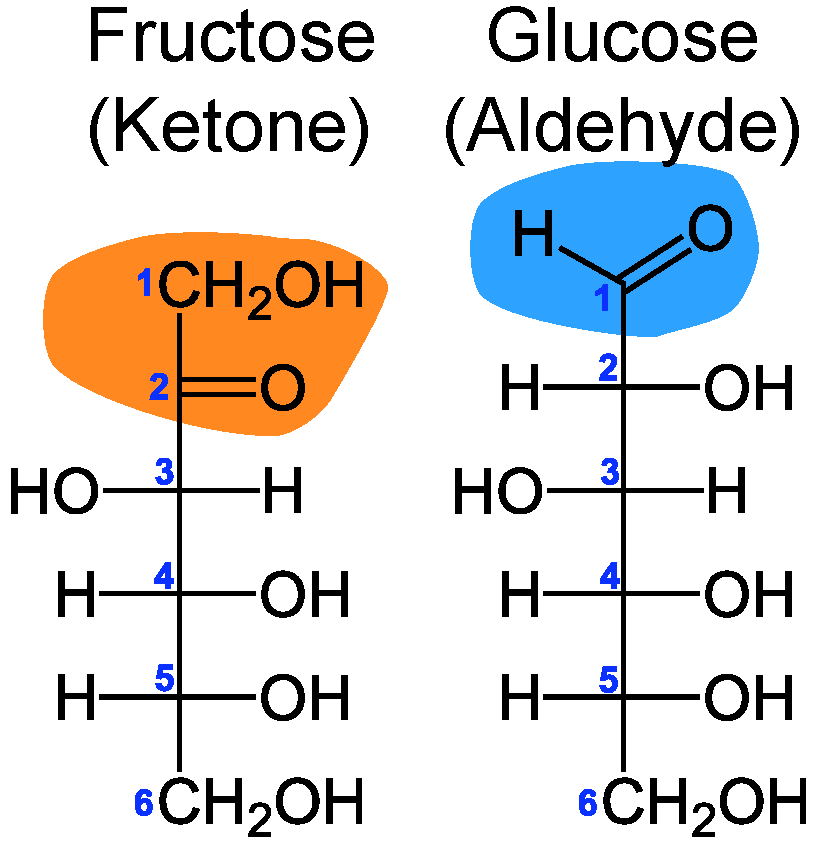
\includegraphics{figures/sugar-aldehydes.png}
\caption{The difference between an aldehyde sugar, and a ketone sugar.}\label{fig:sugar-aldehydes}
\end{marginfigure}

\section{Classes of Carbohydrates}\label{classes-of-carbohydrates}


\newthought{Carbohydrates fall into one of three classes.} The first and simplest class is \textbf{monosaccharides}, often referred to as \textbf{simple sugars}. Monosaccharides include \textbf{glucose, fructose} and \textbf{galactose}. They are found in food sources such as honey, fruits and corn syrup. Typically carbohydrates are not in this simple form in food sources, but during digestion humans break down larger carbohydrates to simple sugars because they are the form of carbohydrates that can be absorbed at the small intestine. Before discussing the larger carbohydrate classes and digestion of carbohydrates, it is important to review the basic CHO nomenclature, chiral nature of the monosaccharide, and a glycosidic bond.\index{Carbohydrates!Monosaccharides}\index{Carbohydrates!Glucose}\index{Carbohydrates!Fructose}\index{Carbohydrates!Galactose}

\subsection{Nomenclature}

The systematic naming of monosaccharides is useful to understand because it can help you visualize the molecular make-up of that carbohydrate unit. An aldehyde will contain the suffix ``\textbf{-ose}'', while a ketone will contain the suffix -\textbf{ulose}. Remember that a carbohydrate is a carbon chain with anywhere from three to seven carbons. Thus, a six- carbon aldehyde carbohydrate is called a hexose, while a six-carbon ketone would be designated as a hexulose. The nomenclature can help to visualize the structure of the carbohydrate, but for the carbohydrates most nutritionally and metabolically relevant, we tend to call them by their trivial names (\textit{e.g.}, glucose, which is technically a hexose).

\subsection{Chirality}

\begin{marginfigure}
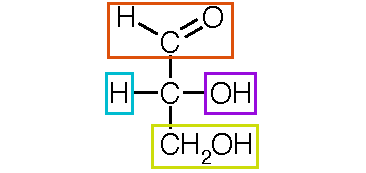
\includegraphics{figures/sugar-chiral.png}
\caption{A triose (glyceraldehyde): the chiral carbon is circled and the four surrounding diverse groups are boxed off.}\label{fig:sugar-chiral}
\end{marginfigure}

We must briefly discuss the stereoisomerism of carbohydrates because most digestive enzymes, metabolic enzymes and transport mechanisms are stereospecific. Carbohydrates are molecules that are optically active, meaning that if a polarized light were to be passed through it, the
light would either rotate to the right (D designation) or the left (L designation). The light rotation is an effect of a \textbf{chiral
carbon} atom in the carbon chain. A chiral carbon is carbon with four \emph{different} groups attached to it.  Glyceraldehyde, a triose, is an example of a carbohydrate containing one chiral carbon (Figure~\ref{fig:sugar-chiral}).\sidenote{Go back to Figure~\ref{fig:sugar-aldehydes} and try to identify how many chiral centers exist in fructose and glucose.}

It is important to note that a carbohydrate with a chain consisting of more than three carbons will have multiple chiral carbons in which the highest numbered chiral carbon will dictate the rotation of the light, thus the D- or L-designation \sidenote{For purposes of this class we will always indicate to you which carbon is the highest numbered}. In other words, glucose, a hexose, can exist in the D-glucose or L-glucose form dependent on the spatial arrangement of the hydroxyl group on its highest numbered chiral carbon (Figure~\ref{fig:sugar-numbering}).

\begin{marginfigure}
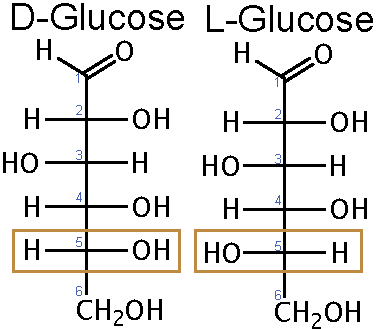
\includegraphics{figures/Glucose-DL.png}
\caption{Representation of the chiral designation of glucose given the hydroxyl direction of the highest numbered chiral carbon.}\label{fig:sugar-numbering}
\end{marginfigure}

\subsection*{Cyclization and Anomeric Forms}

Most monosaccharides with five or more carbon atoms do not exist predominantly in their open-chain (linear) form in solution. Instead, they undergo an intramolecular reaction where a hydroxyl group attacks the carbonyl carbon, forming a \textbf{hemiacetal} (in aldoses) or \textbf{hemiketal} (in ketoses). This cyclization creates a ring structure — typically a six-membered \textit{pyranose} ring (like glucose) or a five-membered \textit{furanose} ring (like fructose).

The carbon that was part of the carbonyl group becomes a new stereocenter called the \textbf{anomeric carbon}\sidenote{I remember this by alpha $\rightarrow$ anchor, beta $\rightarrow$ balloon.}, respectively, of the hydroxyl group (Figure~\ref{fig:sugar-ab}).. Two stereoisomers may form at this carbon:
\begin{itemize}
\item \textbf{$\alpha$-anomer} — the OH on the anomeric carbon is on the opposite side of the ring (trans) from the CH$_2$OH group.
\item \textbf{$\beta$-anomer} — the OH on the anomeric carbon is on the same side (cis) as the CH$_2$OH group.
\end{itemize}

These forms interconvert in solution through a process called \textbf{mutarotation}.

Understanding the anomeric configuration is essential in nutrition because digestive enzymes such as \textit{$\alpha$-amylase} are specific to $\alpha$-1,4-glycosidic bonds (as in starch), and cannot cleave $\beta$-1,4 bonds (as in cellulose). This specificity underlies why cellulose is indigestible in humans.


\newthought{Sugars that can have a free aldehyde or ketone group are called reducing sugars.}\index{Carbohydrates!Reducing Sugars}\index{Maillard Reaction}  All monosaccharides can interchangeably cyclize or decyclize.  As a result at times the ketone or aldehyde group is free and could react with other food components.  One important reaction in cooking is the Maillard reaction where a reducing sugar reacts with an amino group from an amino acid.  This is what gives food its distinctive brown color and creates new flavors.  Note in Figure~\ref{fig:glycosidic-bonds} that when a sugar is part of a disaccharide, oligosacchardie or polysaccharide the aldehyde or ketone may no longer be free, and it can trapped as part of the glycosidic bond.  If both anomeric carbons are part of the glycosidic bond, the compound is no longer a reducing sugar.\sidenote{For example maltose and lactose\index{Carbohydrates!Lactose} are reducing sugars but sucrose is not.  Take a look at their structures and try to understand why this is the case.}


\begin{marginfigure}
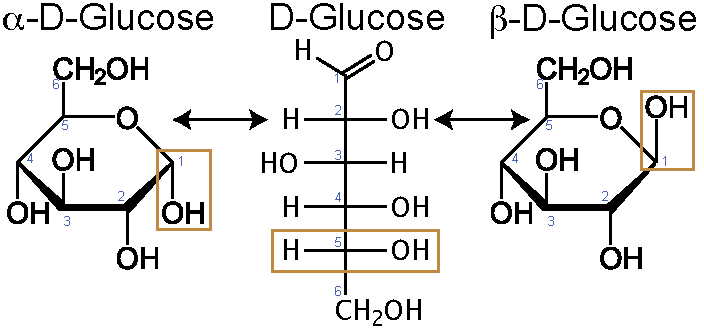
\includegraphics{figures/Glucose-ab.png}
\caption{Cyclization of D-glucose to form alpha or beta-D-glucose.}\label{fig:sugar-ab}
\end{marginfigure}


\subsection{Glycosidic Bonding}\index{Carbohydrates!Glycosidic Bonds |(}

\begin{marginfigure}
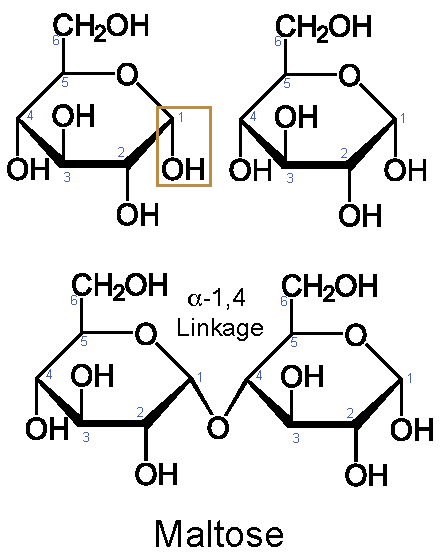
\includegraphics{figures/glycosidic-bonds.png}
\caption{Condensation of two molecules of alpha-D-glucose to form the disaccharide maltose with the glycosidic bond formation designated as alpha 1,4.}\label{fig:glycosidic-bonds}
\end{marginfigure}


\newthought{Glycosidic bonds link monosaccharide units to form oligo- and polysaccharides.} The glycosidic bond is named after the direction (alpha- or beta-) of the hydroxyl group attached to the anomeric carbon, the anomeric carbon number and the carbon number of the subsequent monosaccharide linking the units together (Figure~\ref{fig:glycosidic-bonds}). To form oligo- or polysaccharides through glycosidic bonding, the monosaccharides undergo a reaction that eliminates a water (H\textsubscript{2}0) group called \textbf{condensation} (Figure~\ref{fig:glycosidic-bonds}). Alternatively, the oligo- or polysaccharides can be broken down to their respective monosaccharide units through \textbf{hydrolysis}, or the addition of a water molecule. Hydrolysis\index{Carbohydrates!Hydrolysis} is the key reaction of digestion that will break apart larger carbohydrate units from food into monosaccharide units that are available for absorption at the small intestine.\sidenote{The absorbable unit for carbohydrates in the small intestine is the monosaccaride.}


\section{Disaccharides}\index{Carbohydrates!Disaccharides}

\newthought{Disaccharides are two monosaccharides linked by a glycosidic bond and are the most common type of oligosaccharides found in dietary sources.}
The three major disaccharides in dietary source are maltose, lactose and sucrose\sidenote{If interested, Google dietary sources of maltose, lactose and sucrose. What did you find?}. Maltose consists of two alpha-D-glucose units linked by an alpha 1,4 glycosidic bond (Figure~\ref{fig:glycosidic-bonds}). Lactose contains a beta-D-glucose linked to a beta-D-galactose by a beta 1,4 glycosidic bond\sidenote{This means that the hydroxyl of the animeric carbon is in the beta (balloon) orientation}. Sucrose consists of an alpha-D glucose linked to beta-D fructose by an alpha 1, beta 2 glycosidic bond. The anomeric carbons from both the glucose and fructose units form the glycosidic bond of sucrose, thus there is an alpha- and beta-designation in the glycosidic bond name.

\section{Oligosaccharides}\index{Carbohydrates!Oligosaccharides}

The next class of carbohydrates is oligosaccharides. They contain 2--10 monosaccharide units with each unit linked by a glycosidic bond.  These are less common in our diets but some examples include raffinose (Gal-Glu-Fru, in brussels sprouts, asparagus and cabbage) and stacchyose (Gal-Gal-Glu-Fru, in beans).  We are unable to digest raffinose and stacchyose and therefore are fermented by the microbiota in our large intestine.   Fermentable oligosaccharides are one source of irritable bowel syndrome (IBS), a class of triggers known as FODMAPs\index{FODMAP}\index{Carbohydrates!Raffinose}\index{Carbohydrates!Stacchyose}\sidenote{Also including disaccharides (mainly lactose and sucrose), monosaccharides (primarily fructose), sugar alcohols, and polyols}.  FODMAP elimination diets are a common treatment for IBS, but generally only in the short term as they can result in severe nutrient deficiencies \citep{vanlanenEfficacyLowFODMAPDiet2021}.

\section{Polysaccharides}\index{Carbohydrates!Polysaccharides}

Polysaccharides contain 11 or more and up to 10,000,000 monosaccharide units. The monosaccharide units of the polysaccharide can be the same (homopolysaccharide) or can have varying monosaccharide units  (heteropolysaccharide). Another characteristic of polysaccharides is their degree of branching\index{Carbohydrates!Branching}. Some are linear and contain zero branching units while others have varying degrees of branching. Typically, the more branching the more water-soluble the polysaccharide is (see Fiber reading for more information on water-solubility and polysaccharides). The branching also becomes important for storage capacity, which we will discuss in more detail when we talk about specific polysaccharides in the following subsections. There are three polysaccharides we will discuss that have relevant implications in human nutrition --- starch, glycogen and cellulose. Common among these three polysaccharides is that they are all homopolysaccharides containing only glucose units.

\newthought{Starch is the most abundant polysaccharide found in plants} (\textit{e.g.}, tubers, seeds, roots, some fruits). Starch is found in two forms, \textbf{amylose}\index{Carbohydrates!Amylose} and \textbf{amylopectin}\index{Carbohydrates!Amylopectin}. Amylose is linear, unbranched and made of alpha-D-glucose connected by an alpha 1,4 glycosidic bond. Amylopectin is moderately branched and a homopolymer of alpha-D-glucose linked by alpha 1,4 bonds on the linear chains but by alpha 1,6 bonds at the branching points. The typical length of a linear  between branching points of amylopectin is 20--25 glucose units. In uncooked food sources containing starch, the linear structure of amylose allows it to be tightly packed. This creates a structure that is not as readily digestible as the branched, less packed structure of amylopectin. In contrast, the processing and heating of amylose-containing foods (i.e., cooking) can loosen hydrogen bonds within the structure making it more accessible for digestion.\sidenote{\textbf{Reflection}:Have you ever eaten flax seeds? Think of how well your body was able to digest ground (``processed'') flax seeds compared to whole flax seeds.}

\newthought{Cellulose is a linear homopolymer of $\beta$-D glucose linked by $\beta$ 1,4 bonds.} This bond arrangement is significant in the digestive
tract because digestive enzymes are not specific to this organization, thus cellulose is non-digestible (further explanation in Digestion section and Fiber reading) and is an insoluble fiber source. Like amylose, the linear structure allows cellulose to be highly packed within plant cell walls, thus cellulose is key for the structural stability of plant cell walls.\index{Carbohydrates!Cellulose}.  Insoluble fibers such as cellulose add bulk to stool and help to regulate bowel movements.


\newthought{glycogen is a highly branched, homopolymer of $\alpha$-D-glucose.} Glycogen\index{Carbohydrates!Glycogen} is abundant in skeletal muscle and liver tissue of mammals. The glucose units are linked by $\alpha$ 1,4 bonds on the linear chains but by $\alpha$ 1,6 bonds at the branching points (just like amylopectin). The typical length of a linear chain between branching points is 10--14 glucose units producing a higher molecular weight compound compared to amylopectin. The highly branched structure of glycogen allows for increased storage capacity in mammal tissue. More branching also allows for a higher degree of accessibility for metabolic enzymes, thus glycogen is a ready source of energy for humans (and other mammals).\  \sidenote{\textbf{Reflection}: Pause and summarize (\textit{e.g.}, in a table format) either the make- up of the three disaccharides or the three types of polysaccharides that we discussed. Compare and contrast.}\index{Carbohydrates!Glycosidic Bonds |)}\index{Carbohydrates!Structure |)}. Glycogen as a major storage form of glucose can support blood glucose in a healthy individual for 12-24 hours, depending on the individual and their activity level \citep{hortonProlongedFastingSignificantly2001}.  

\bibliography{library}
\bibliographystyle{plainnat}

\end{document}
